% Moved verbatim from Paper A (new/sections/example.tex lines 3-12 (Fig. 1 with srcSlice-Q's classical lines), commit f96523f) on 2026-10-29. Raw material for Paper B; rewrite, do not reuse.
\begin{figure}[t]
  \centering
  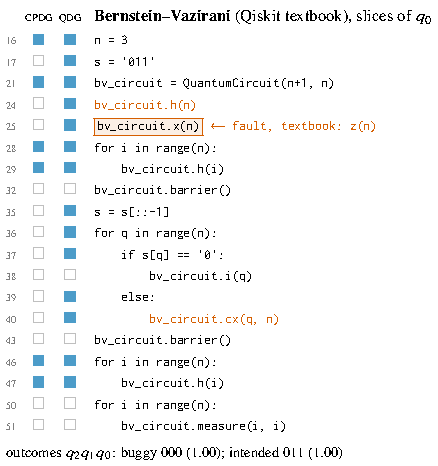
\includegraphics[width=\columnwidth]{figures/fig_bv.pdf}
  \caption{The Bernstein--Vazirani program of the Qiskit textbook~\cite{qiskittextbook}, with comments and blank lines
  omitted and the textbook's line numbers kept. Line~25 carries a seeded fault, \texttt{x(n)} where the textbook
  applies \texttt{z(n)}. The two columns mark the lines in the backward slice of $q_0$ under the classical PDG and
  under the QDG. The classical slice misses the orange lines, which can change $q_0$. Slices are computed statically
  by \tool{}, and outcomes and dependences by the study's code.}
  \label{fig:bv}
\end{figure}
